\section{Adjacent technologies}
%\subsection{Definition}

As mentioned in the previous section, the Internet of Things (IoT) has evolved rapidly. technology that connects devices and sensors to the internet, so The success of any IoT project depends on the integration of a range of adjacent technologies,such as  wireless sensor networks, RFID, remote sensing, NFC, video surveillance ... etc \\
These technologies are essential for collecting and processing data from IoT devices, enabling make intelligent decisions and maintain the security and confidentiality of the data generated and transmitted by IoT devices.\\
In this section, we explore the technologies that are closely related to IoT, including Remote Sensing and RFID Technology\\


\subsection{RFID Radio Frequency IDentification Technology}

\subsubsection{Definition}
The RFID (Radio Frequency IDentification) technology also well-known as wireless radio frequency identification,non-contact card and inductive electronic chip or electronic tag . is a wireless (contactless) application known to the traceability, access control and logistics. It became ubiquitous in industry and our daily life (ticketing, payment, passports, car keys, etc.).RFID nowadays is a standardized technology. can offer many advantages, such as unitary, identification, wireless communication, and low cost of tags.\cite{duroc2018rfid}\\

\subsubsection{RFID Systems Structure And Main Components}
%\subsubsection*{*}
RFID systems are generally divided into two layers, physical layer and Information Technology (IT) layer.
The figure below shows the RFID systems architecture and main components:\\
\begin{figure}[h]
	\centering
	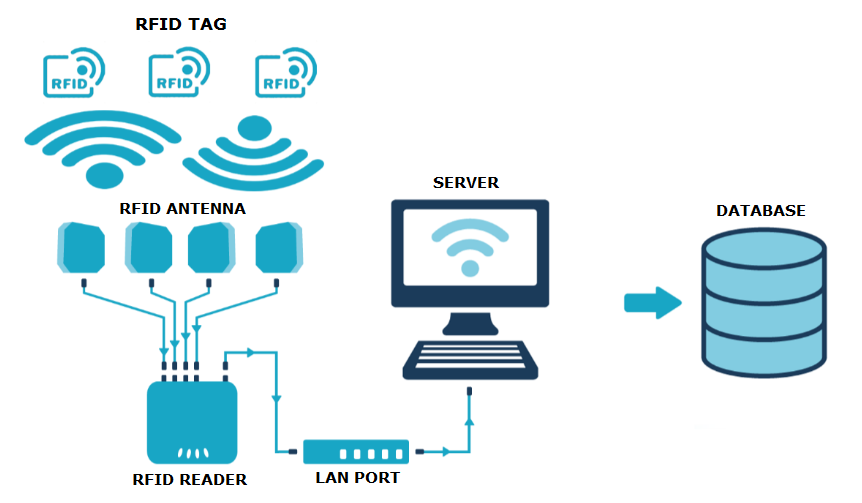
\includegraphics[width=0.8\textwidth,height=0.3\textheight]{images chap1/rfidsys}
	\caption{General RFID system Structure and Main Components }\cite{rfidsys}
\end{figure}

\textbf{physical layer composed of :}
\begin{itemize}
	\item One or more RFID tag or transponder (transmitter/responder), which is consisting of a semi-conductor chip, a contact or contactless wire, and in some cases coupled with a battery.\\
	\item  One or more reader or a read/write gadget(also called an investigator), which is consisting of a RF receiver that typically connected to the reader antenna, and a control hardware module.\\
	\item  A controller connected with PC or a workstation where the data sorted in a database and software controller (middleware).
	\item One or more reader antennas
\end{itemize}
\textbf{Information Technology (IT) layer which consist :}
\begin{itemize}
	\item One or more host computers (or servers) connected to readers (directly or through a network)
	\item Appropriate software (device drivers, filters, middleware, databases, and user applications)
\end{itemize}

% a reader with integrated or external connected antenna, an electronic tag (transponder), and a compute device that hosts a database and an application dependent software package and an application software system. \cite{duroc2018rfid}\\%
%\begin{picture}
%\includegraphics[\textwidth]{rfidsystem}
%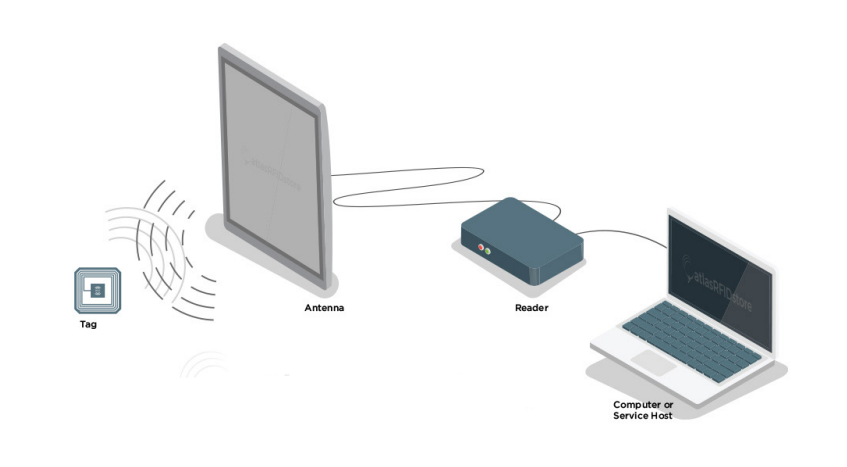
\includegraphics{rfidSystem}
%\end{picture}}
\subsubsection{RFID Work Concept}
Radio frequency identification (RFID) is a type of automatic identification and data capture methods of identifying objects  using radio waves, without the need for physical contact. RFID utilizes radio frequencies to enable two-way communication between a reader and an electronic tag or radio frequency card, allowing for the exchange of data and identification of the object.\cite{li2018flooding}\cite{landaluce2020review}\\

\begin{figure}[h]
	\centering
	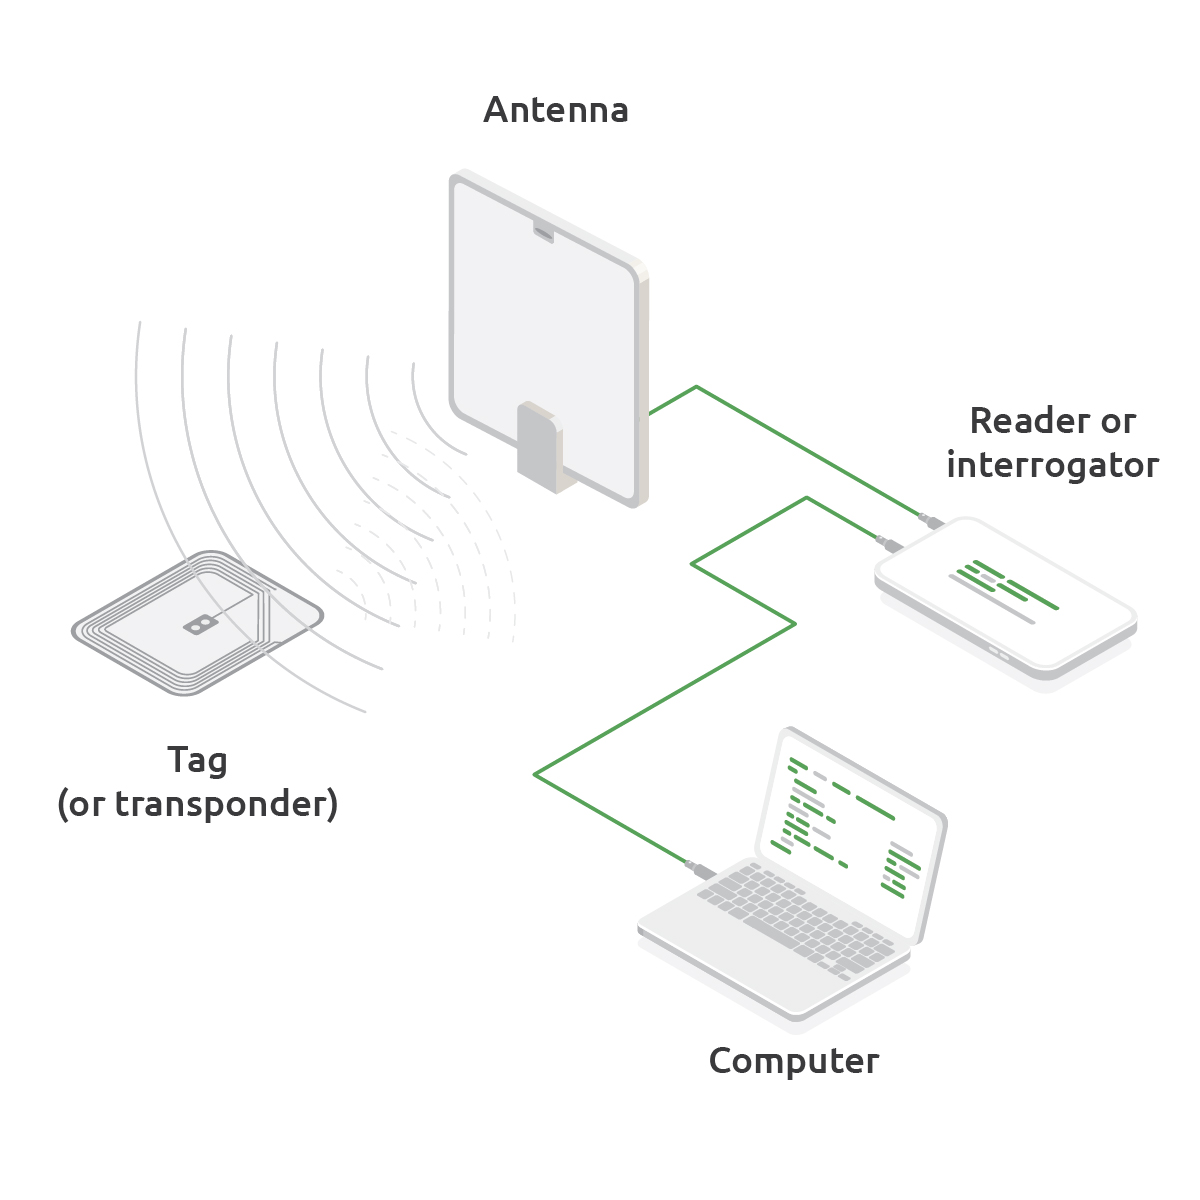
\includegraphics[width=0.8\textwidth,height=0.3\textheight]{images chap1/r}
	\caption{General RFID system Structure and Main Components }\cite{rfidwork}
\end{figure}

This process functions as follows :\cite{li2018flooding}
\begin{itemize}
	\item An RFID system involves attaching a tag to an object, which stores information about the object.
	\item The reader is responsible for powering the tag (just in the passive tag case), identifying it, and reading/writing data from/to the tag.
	\item Additionally, the reader communicates with a database to process information from the tags.
	\item When an object that has an RFID tag on it comes within range of the reader, the reader transmits a radio signal to the tag.
	\item The tag then powers up and sends its information back to the reader, sometimes receiving new information from the reader.
	\item The information is then sent to a database for processing.
	
\end{itemize}
Note : the RFID reader powered only the tags of passive type , the other tag type are powered by other ways.\cite{li2018flooding}\\
Note : since RFID systems use radio waves, the reader's antenna can communicate with the tag without requiring a direct line of sight between them.\cite{li2018flooding}

\subsubsection{RFID System Classification :}
%\subsubsection{RFID System classification}
The RFID systems can be classified based on many parameters such as Power, communication range, data processing, programming, and protocol\cite{duroc2022identification} .the main classification criteria are :\\\textbf{A) according to the RFID tag type (power source of the tags):}\\
RFID tag can be classified according to their power supply source as follows :\\
\begin{itemize}
	
	
	\item \textbf{ Active tags:} These tags have an embedded battery that enables them to emit a signal without needing to be remotely powered. They can achieve reading distances of a few meters and are primarily used for sending large amounts of information over long distances. However, they are more expensive than other systems, require maintenance service, and are less integrated.\cite{chawla2007overview}
	\item \textbf{ Semi-passive tags (also known as semi-active):} These tags are powered by an embedded energy source similar to active tags, but the battery is used to store data between successive communication exchanges rather than sending a signal. Semi-passive tags use backscattering techniques to send back the reader signal and are often used for recording data during goods transporting. They are particularly useful in food traceability and logistic traceability applications that require temperature monitoring and equipment fleet surveillance.
	\item \textbf{ Passive tags:} These are the most commonly used RFID tags due to their low cost, miniature size, and simplicity of architecture. They do not include a battery or RF transceiver like semi-passive and active tags. Instead, they use backscattering techniques to respond to reader commands. A passive tag receives the power needed to operate from the wave incident from the reader. They are compact, simple, and composed of an antenna for communicating with the reader and an electronic chip that integrates memory for storing data to be transmitted.this type of tags are commonly used in stock tracking and the supply chain management applications.
\end{itemize}
\begin{figure}[h]
	\centering
	\includegraphics[width=0.8\textwidth,height=0.25\textheight]{images chap1/rfidpa}
	\caption{RFID tag types }\cite{rfidtype}
\end{figure}

According to the communication distance RFID passive tags can be divided into near-field and far-field. 
For this reason, the data exchange mode between the read/write device and the electronic tag is correspondingly divided into load modulation and backscatter modulation.\cite{rfidpascla}\\

\textbf{B) according to the frequency bands in which the system operate:} \\RFID systems work from Low frequency (LF) to Super (Ultra) High frequency (SHF/UHF),these frequencies have been normalized to avoid interference by other devices of other technologies.\cite{duroc2018rfid} \\
1) Low Frequency\\
2) High Frequency\\
3) Ultra-High Frequency
%4) Microwaves
\begin{figure}[h]
	\centering
	
	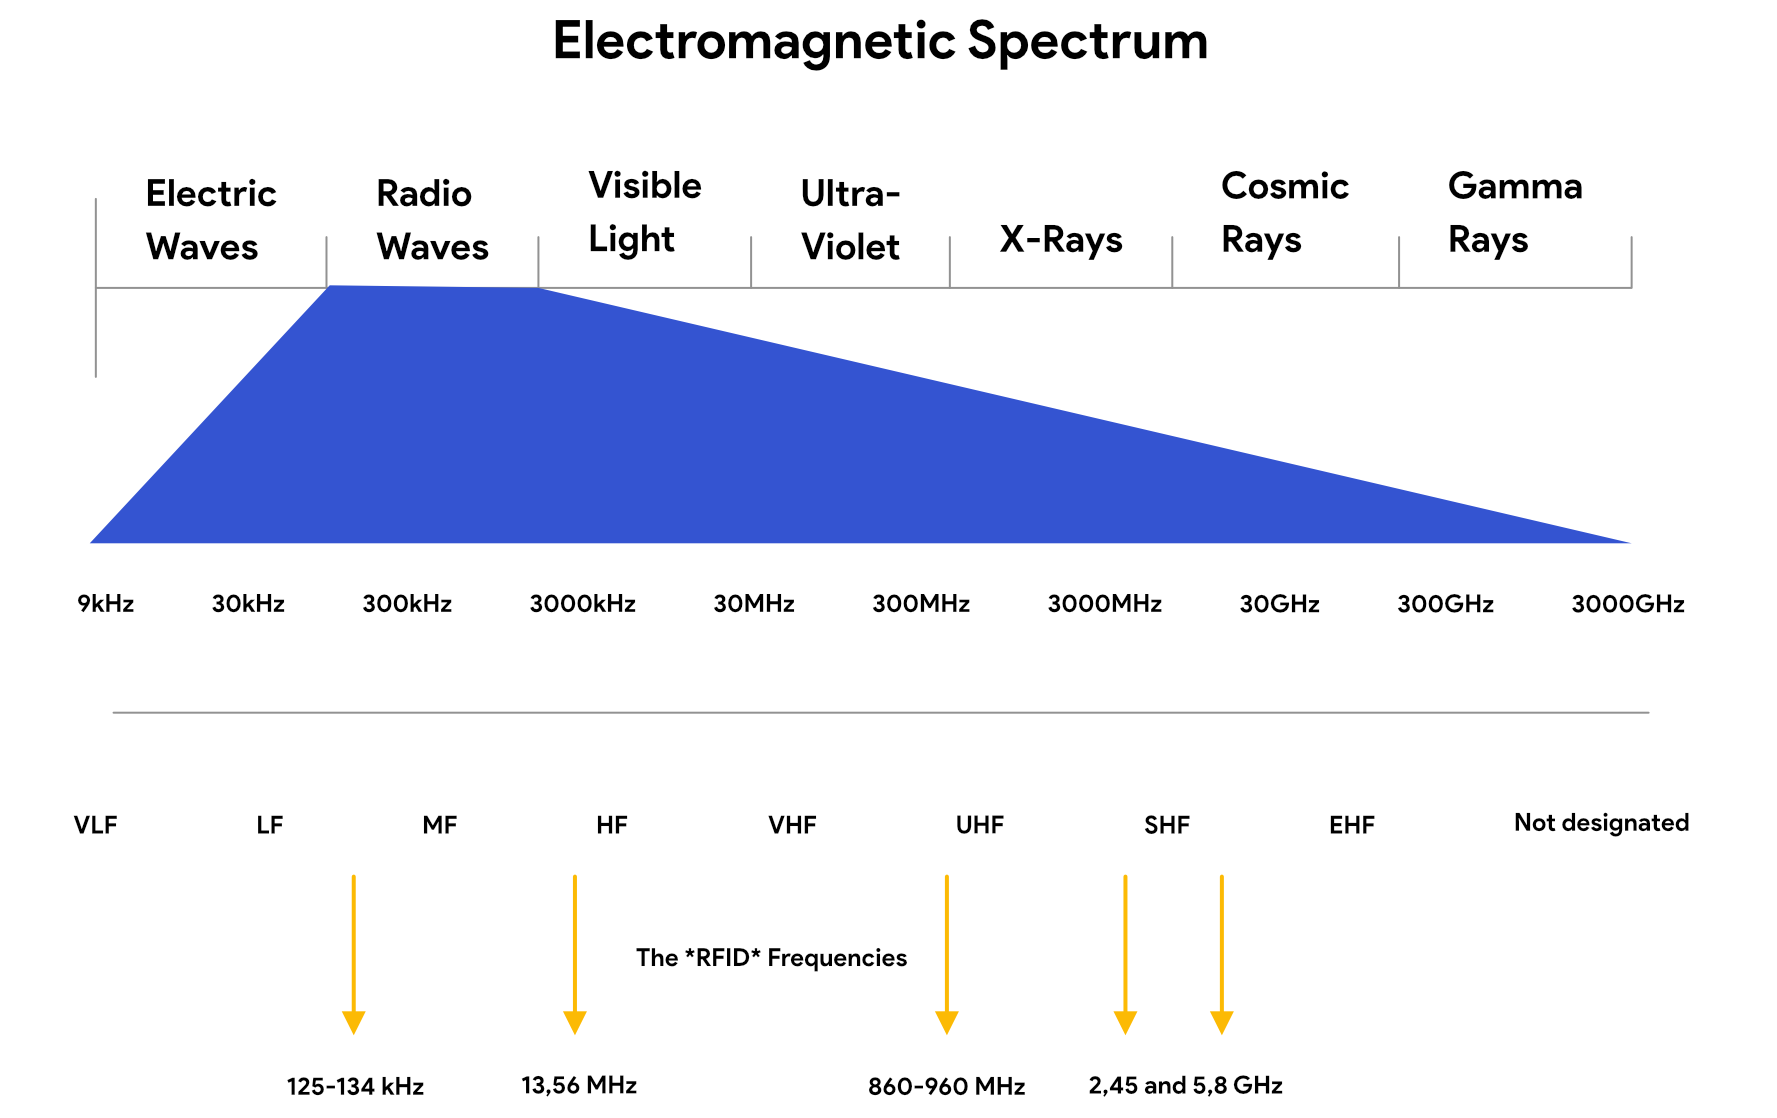
\includegraphics[width=0.9\textwidth ,height=0.3\textheight]{images chap1/rfidfreqs}
	\caption{RFID frequencies in the electromagnetic spectrum}\cite{rfidfreqs}
\end{figure}

we have summarized the most common and frequently used operating frequencies by RFID systems and examples of application in different humanity services in the following table \\
\begin{table}[h]
	
	\centering
	\begin{tabular}{|p{2cm}|p{2cm}|p{1cm}|p{3cm}|p{2.5cm}|p{4cm}|}
		\hline
		frequency &Frequency Range&Read Range&Coupling Type&Existing Standards&Application At The Service Of Humanity\\ \hline
		LF (Passive Tags)&125 khZ 134 KHz &about 0.1 m&Magnetic
		Near field&11784/85, 14223, 18000-2&Smart card, ticketing, access, animal tagging, laundry…\\ \hline
		HF (Passive Tags)&13.56 MHz&about 1 m&Magnetic Near field&18000-3.1, 15693, 14443A, B, C&Small item management, supply chain, anti-theft, library…\\ \hline
		UHF (Passive Tags)&900 MHz 902–928 MHz US
		868–871 MHz Europe
		950–956 MHz Asia&in range 2–20 m&Electromagnetic 
		Far field &EPC C0, C1, C1G2, 18000-6&Transportation vehicle ID, access, security, supply chain, large item management…\\ \hline
		Microwaves (Active Tags)&2.4 GHz  5.8GHz&about 10 m&Electromagnetic Far field&18000-4&Transportation vehicle ID, road toll, access, security, supply chain, large item management…\\ \hline
		
	\end{tabular}
	\caption{RFID Operating Frequencies} 
\end{table}




\subsection{Remote Sensing Technology}
\subsubsection{Definition}
Remote sensing is a technology that allows us to gather information on the Earth's surface and  environment remotely .This can be done using a variety of different sensors, such as cameras; radars, Lidar(Light Detection and Ranging), sonars, lasers,  seismographs or gravimeters. \cite{girard2018processing}\\
\subsubsection{Work Concept}
Remote sensing is a type of data acquisition method typically by using the measurement of electromagnetic radiation emitted or reflected from objects studied in a certain frequency range (infrared, visible, microwaves).\\this is made possible by the fact that the objects studied (plants, houses, water surfaces or air masses) emit or reflect radiation at different wavelengths and intensities depending on their condition. Some remote sensing instruments use sound waves in a similar manner, while others measure variations in magnetic or gravitational fields.\cite{denis2020travaux}

By analyzing the collected data from the sensors, we can gain insights into a wide range of applications, including natural resource management, urban planning, and environmental monitoring like land use, vegetation health, weather patterns, and more.\cite{mather2016classification}
\subsubsection{Types Of Remote Sensing Systems}
Here we mention most common Remote Sensing types: \cite{elachi1988spaceborne}
\begin{itemize}
	\item 	Visual Remote Sensing System (e.g., human visual system)
	\item 	Optical Remote Sensing
	\item 	Infrared Remote Sensing
	\item 	Microwave Remote Sensing
	\item 	Radar Remote Sensing
	\item 	Satellite Remote Sensing
	\item 	Airborne Remote Sensing
	\item 	Acoustic and near-acoustic Remote Sensing
\end{itemize}


\subsubsection{Types Of Sensors In Remote Sensing Systems}
There are two major types of sensors, passive and active, that represent the basic difference between remote sensing systems.\cite{zhou2021potential}\cite{heisig2022predicting}
\begin{itemize}
	\item \textbf{Passive Remote Sensing }\\
	Passive remote sensing records natural radiation from Earth's surface or atmosphere.the Sunlight is the most common source of radiation that is reflected from Earth's surface.\\
	Passive sensors used in remote sensing include radiometers and spectrometers. these sensors operate in different parts of the electromagnetic spectrum,they can measure signals across several spectral bands simultaneously.\\\cite{tong2019trends}
	Images produced from these sensors provide important information about the Earth's surface and atmosphere.those images can help understand physical characteristics of the Earth, such as surface temperature and geological properties.
	An example of a passive sensor is a camera with the flash turned off.
	this method have limitations with cloud cover but provides true-color images.\cite{schroeder2019passive}
	
	\item \textbf{Active Remote Sensing }\\
	Active remote sensing uses active sensors to emit radiation towards a target and then measure the reflected or backscattered radiation.Active sensors include LiDAR, RADAR, scatterometers, and altimeters, which mostly operate in the microwave band of the electromagnetic spectrum.\\
	Active sensors are immune to weather conditions and can function in the dark ,so they can be used in various fields, such as volcanology, forestry, and glaciology.
	As an example Synthetic-Aperture Radar (SAR) technology can penetrate through vegetation to obtain surface layer information.\\
	this method main disadvantage is that the pulse power can interfere with other sources of radiation, requiring additional processing and analysis for clear interpretation.\cite{zhou2021potential}
\end{itemize}
\begin{figure}[h]
	\centering
	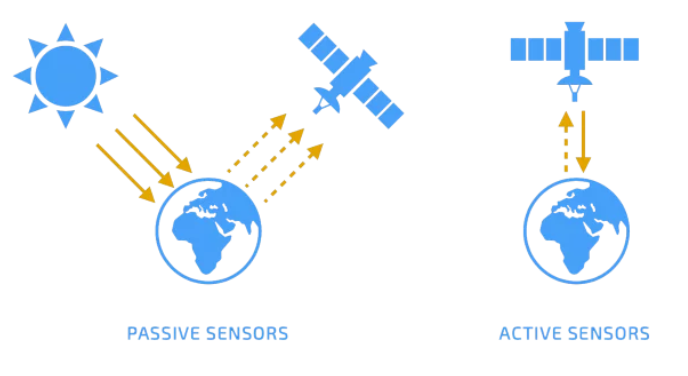
\includegraphics[width=0.7\textwidth ,height=0.3\textheight]{images chap1/rspa}
	\caption{Passive vs Active remote sensing approaches}\cite{rsap}
\end{figure}

\subsubsection{Integration With IoT:}

The integration of remote sensing with IoT technologies can create smart sensing systems that are more efficient and effective. For example, in precision agriculture, remote sensing can be used to collect data on crop health, soil moisture, and other factors, which can be fed into an IoT platform to automatically adjust irrigation or nutrient levels. In disaster management, remote sensing can be used to track the spread of wildfires or floods, while IoT sensors can be used to monitor air quality or track the movement of people and vehicles. In smart cities, remote sensing can be used to monitor traffic patterns, while IoT sensors can be used to monitor air quality, noise levels, and other environmental factors.\cite{ullo2021advances}

\subsubsection{Remote Sensing Applications}
there are a several fields that can integrate remote sensing technology such as :
\begin{itemize}
	\item 	\textbf{Precision agriculture:} Remote sensing can be used in IoT-enabled precision agriculture to monitor crop growth and detect early signs of disease or nutrient deficiency. This can help farmers optimise their harvests and reduce the use of resources. 
	
	\item 	\textbf{Environmental monitoring:} Remote sensing can be used to monitor the health of the environment, including air quality, water quality, and natural disasters. This can be especially helpful in areas subject to pollution or exposed to natural disasters.
	
	\item 	\textbf{Infrastructure monitoring:} Remote sensing can be used to monitor the health and safety of infrastructure such as bridges, dams, and pipelines. This can help identify potential structural issues before they become critical and avoid expensive repairs.
	
	\item 	\textbf{Wildlife conservation:} Remote sensing can be used to monitor wildlife habitats and detect changes in wildlife behavior. It can help environmentalists better understand the needs of animals and take measures to protect them.
	
	\item 	\textbf{Smart cities:} Remote sensing can be used in IoT-enabled smart cities to monitor traffic patterns, energy consumption, and air quality. This enables cities to optimize their resources and enhance the quality of life of their citizens.
	
	\item \textbf{Monitoring crop health and growth:} in agriculture field Remote sensing can be used to track plant growth, detect disease or nutrient deficiencies, and assess overall crop health. This can help farmers make more informed decisions about irrigation, fertilization, and pest control. \cite{schulz2018machine}\cite{chong2017review}\cite{navalgund2007remote}\cite{karthikeyan2020review}
\end{itemize} 
%figure mrygla H hi rasmi
%\begin{figure}[H]
%	\centering
%	\includegraphics[width=0.3\textheight]{rfidpa}
%	\caption{passive and active}
%\end{figure}